\chapter{Аналитический раздел}

\section{Постановка задачи}
В соответствии с заданием целью данной работы является разработка программного комплекса, состоящего из программы уровня пользователя, получающей информацию о конкретном процессе, и драйвера символьного дисплея, обеспечивающего вывод информации, заданной приложением.

В ходе работы необходимо решить следующие задачи:
\begin{enumerate}
	\item Провести сравнительный анализ способов реализации драйверов устройств.
	\item Сделать выбор способа реализации драйвера символьного дисплея.
	\item Описать способ получения информации о процессе по его идентификатору из пространства пользователя.
	\item Провести сравнительный анализ существующих интерфейсов взаимодействия с символьным жидкокристаллическим дисплеем.
	\item Сделать выбор интерфейса взаимодействия с символьным жидкокристаллическим дисплеем в соответствии с поставленной целью.
	\item Сделать выбор системных вызовов, поддерживаемых драйвером, в соответствии с поставленной целью.
	\item Разработать алгоритмы и структуру ПО.
	\item Реализовать драйвер символьного дисплея для вывода информации о конкретном процессе как загружаемый модуль ядра Linux.
	\item Реализовать программу уровня пользователя для взаимодействия с символьным дисплеем.
\end{enumerate}

\section{Способы реализации драйверов устройств}
Драйвер устройства~---~программа, управляющая работой внешнего устройства со стороны системы. Существуют драйверы уровня пользователя и драйверы в формате загружаемого модуля ядра.
\begin{enumerate}
	\item Драйверы уровня пользователя предоставляют интерфейс между приложениями и драйверами уровня ядра. Например, драйверы принтеров.
	\item Драйверы уровня ядра выполняются на уровне ядра, используя его структуры и функции. Обычно такие драйверы разделяются на подуровни. В основном верхние уровни получают информацию от приложений, обрабатывают ее и передают драйверам нижнего уровня. К этой категории относятся, например, драйверы файловых систем. 
\end{enumerate}

\section{Выбор способа реализации драйвера символьного дисплея}
В UNIX-системах для обращения к драйверу, реализованному как загружаемый модуль ядра, используются специальные файлы устройств. Специальные файлы устройств в действительности являются только указателями на соответствующие драйверы устройств в ядре. Каждому устройству соответствует хотя бы один специальный файл. Обычно они лежат в каталоге \texttt{/dev} корневой файловой системы. За счет этого обеспечивается унифицированный доступ к периферийным устройствам~---~с ними можно взаимодействовать, как с обычными файлами: открывать, закрывать, читать, писать. Поэтому в данной работе было принято решение реализовать драйвер устройства как загружаемый модуль ядра. 

\section{Способ получения информации о процессе по его PID из пространства пользователя}
Виртуальная файловая система \texttt{proc} не является монтируемой файловой системой поэтому и называется виртуальной. Её корневым каталогом является каталог \texttt{/proc}. Основная задача файловой системы \texttt{proc}~---~предоставление информации процессам о занимаемых ими ресурсах, что совпадает с поставленной в работе целью.

Каждый процесс в файловой системе \texttt{proc} имеет поддиректорию: \texttt{/proc/<PID>}. В данной директории находятся файлы и другие вложеные директории, содержащие информацию о данном процессе. 

В данной работе будут использованы:
\begin{enumerate}
	\item cmdline~---~файл, содержащий командную строку запуска процесса;
	\item fd~---~директория, содержащая ссылки на файлы, открытые процессом;
	\item tasks~---~директория, содержащая поддиректории потоков;
	\item stat, statm~---~файлы, содержащие информацию о состоянии процесса;
	\item comm~---~файл, содержащий имя исполняемого файла процесса.
\end{enumerate}

\section{Интерфейсы взаимодействия с внешними устройствами}

\subsection{Последовательная и параллельная связь}
Для взаимодействия между устройствами должен быть определен протокол связи. Выделяется 2 основных вида связи:
\begin{enumerate}
	\item Последовательная.
	\item Параллельная.
\end{enumerate}

Последовательная связь может быть реализована с использованием меньшего количества проводов, однако требует настройки механизма синхронизации~\cite{bib4} и обеспечивает меньшую скорость передачи по сравнению с параллельной~\cite{bib7}. Также, последовательная связь является наиболее широко используемой коммуникационной методологией. Исходя из данных особенностей, был выбран последовательный вид связи, и далее будут рассмотрены поддерживающие его интерфейсы.

\subsection{SPI}
Интерфейс SPI представляет собой последовательный четырехканальный интерфейс синхронной передачи данных~\cite{bib5}. В SPI передача данных синхронизирована с тактовым сигналом основного устройства. Периферийные устройства синхронизируют получение битовой последовательности с тактовым сигналом. К одному интерфейсу ведущего устройства может подключаться несколько периферийных устройств. Ведущее устройство обрабатывает все данные и выбирает ведомое для передачи. Периферия, не выбранная ведущим устройством, не принимает участия в передаче по SPI. Шина SPI способна передавать информацию сразу в двух направлениях, стандартная скорость обмена данными до 20 Мбит/с.

Преимущества интерфейса SPI:
\begin{enumerate}
	\item Надежность синхронного типа связи.
	\item Возможность подключения нескольких периферийных устройств.
	\item Скорость передачи данных выше, чем у UART и I2C.
\end{enumerate}

Недостатки интерфейса SPI:
\begin{enumerate}
	\item Требуется минимум 4 линии связи, количество каналов растёт при увеличении числа подключаемых устройств.
	\item Только ведущий контролирует весь процесс коммуникации, нет прямой связи между ведомыми.
\end{enumerate}

\subsection{UART}
Интерфейс UART обепечивает последовательную асинхронную связь. UART работает путем перевода между параллельной связью и последовательной связью~\cite{bib7}. Поддерживает дуплексный режим. Наиболее распространённые скорости передачи~---~до 112 Кбит/с.

Необходимо только два провода. Поскольку связь асинхронная, оба взаимодействующих устройства должны использовать свои независимые внутренние системы тактирования для функционирования. Тем не менее, существует термин «скорость передачи», который помогает этим устройствам оставаться в режиме синхронизации, фиксируя скорость обмена данными. Скорость передачи данных в бодах равно число бит данных, передаваемое в секунду, поэтому оба устройства должны работать с одинаковой скоростью передачи, чтобы поддерживать его надлежащее функционирование. Время согласовывается заранее между обеими единицами, и к каждому пакету данных добавляются специальные биты~---~слово. UART используют эти биты для синхронизации друг с другом. Интерфейс UART имеет большое ограничение, связанное с тем, что только два устройства могут обмениваться данными с помощью этого протокола одновременно.

Преимущества интерфейса UART:
\begin{enumerate}
	\item Обеспечивается наличие различных скоростных режимов передачи, что делает протокол практически универсальным.
	\item Является одной из самых простых форм последовательной связи.
\end{enumerate}

Недостатки интерфейса UART:
\begin{enumerate}
	\item Одновременно могут быть подключены только два устройства.
	\item Требуется передача дополнительных битов для согласования времени передачи.
	\item Скорость передачи данных ниже, чем у I2C и SPI.
\end{enumerate}


\subsection{I2C}
Интерфейс I2C обепечивает последовательную синхронную связь~\cite{bib6}. Данные передаются по двум линиям: данных и тактирования. Обе линии поддерживают дуплексный режим. Устройства, участвующие в транзакциях, разделяются на ведущее устройство и ведомые им устройства. Ведущее определяет начало и конец обмена данными, синхронизирует транзакции и опрашивает ведомые устройства. Максимальное количество периферийных устройств для подключения к шине~---~127. Данные по шине I2C могут передаваться со скоростью до 100~--~200 Кбит/с в стандартном режиме, и до 400 Кбит/с в быстром режиме.

Каждая посылка данных состоит из 8 бит данных, формируемых передатчиком. Приемник во время девятого такта формирует бит подтверждения, по которому передатчик убеждается, что передача прошла успешно. После передачи бита подтверждения ведомое устройство может начать следующую передачу.

Преимущества интерфейса I2C:
\begin{enumerate}
	\item Необходимо 2 линии связи, независимо от количества подключенных устройств.
	\item Возможность подключения нескольких ведущих устройств.
	\item Протокол I2C является более стандартизованным, поэтому, пользователь более защищен от проблем несовместимости выбранных компонентов.
	\item Позволяет взаимодействовать на одной шине устройствам с различным быстродействием интерфейсов.
\end{enumerate}

Недостатки интерфейса I2C:
\begin{enumerate}
	\item Скорость передачи данных ниже, чем у SPI, из-за большого количества операций с кадрами данных.
\end{enumerate}

\section{Выбор интерфейса взаимодействия с символьным жидкокристаллическим дисплеем}

В таблице \ref{table:cmp_int} приведен сравнительный анализ рассмотренных интерфейсов взаимодействия с внешними устройствами.

\begin{table}[h]
\begin{center}
\caption{\label{table:cmp_int} Сравнительный анализ рассмотренных интерфейсов взаимодействия с внешними устройствами}
\begin{tabular}{|c|cccc|}
\hline
\multirow{2}{*}{\begin{tabular}[c]{@{}c@{}}Интерфейсы\\ взаимодействия\\ с внешними\\ устройствами\end{tabular}} & \multicolumn{4}{c|}{Критерии сравнения}                                                                                                                                                                                                                                                                                                                          \\ \cline{2-5} 
& \multicolumn{1}{c|}{\begin{tabular}[c]{@{}c@{}}Скорость\\ передачи\\ данных\\ (до Кбит/с)\end{tabular}} & \multicolumn{1}{c|}{\begin{tabular}[c]{@{}c@{}}Кол-во\\ каналов\\ (мин.)\end{tabular}} & \multicolumn{1}{c|}{\begin{tabular}[c]{@{}c@{}}Надежность\\ передачи\end{tabular}} & \begin{tabular}[c]{@{}c@{}}Требует\\ передачи\\ доп. данных\end{tabular} \\ \hline
UART                                                                                                             & \multicolumn{1}{c|}{112}                                                                                & \multicolumn{1}{c|}{2}                                                                 & \multicolumn{1}{c|}{–}                                                             & +                                                                        \\ \hline
SPI                                                                                                              & \multicolumn{1}{c|}{20 480}                                                                             & \multicolumn{1}{c|}{4}                                                                 & \multicolumn{1}{c|}{+}                                                             & –                                                                        \\ \hline
I2C                                                                                                              & \multicolumn{1}{c|}{200}                                                                                & \multicolumn{1}{c|}{2}                                                                 & \multicolumn{1}{c|}{+}                                                             & –                                                                        \\ \hline
\end{tabular}
\end{center}
\end{table}

В результате сравнения было принято решение использовать интерфейс I2C, так как он является более надежным, не требует большого числа каналов и передачи дополнительных данных. Скорость передачи не являлась ключевым критерием в соответствии с целью работы, поэтому, несмотря на то, что SPI превосходит I2C по этому критерию, он, как требующий наличия большего числа каналов, не был выбран.

\section*{Вывод}
Было принято решение реализовать драйвер символьного дисплея для вывода информации о процессе как модуль ядра Linux. Также, был проведен сравнительный анализ интерфейсов взаимодействия с внешними устройствами, в результате которого был выбран интерфейс I2C.

%\newpage
%
%\begin{table}[h!]
%  \centering
%  \begin{tabular}{p{1\linewidth}}
%    \centering
%    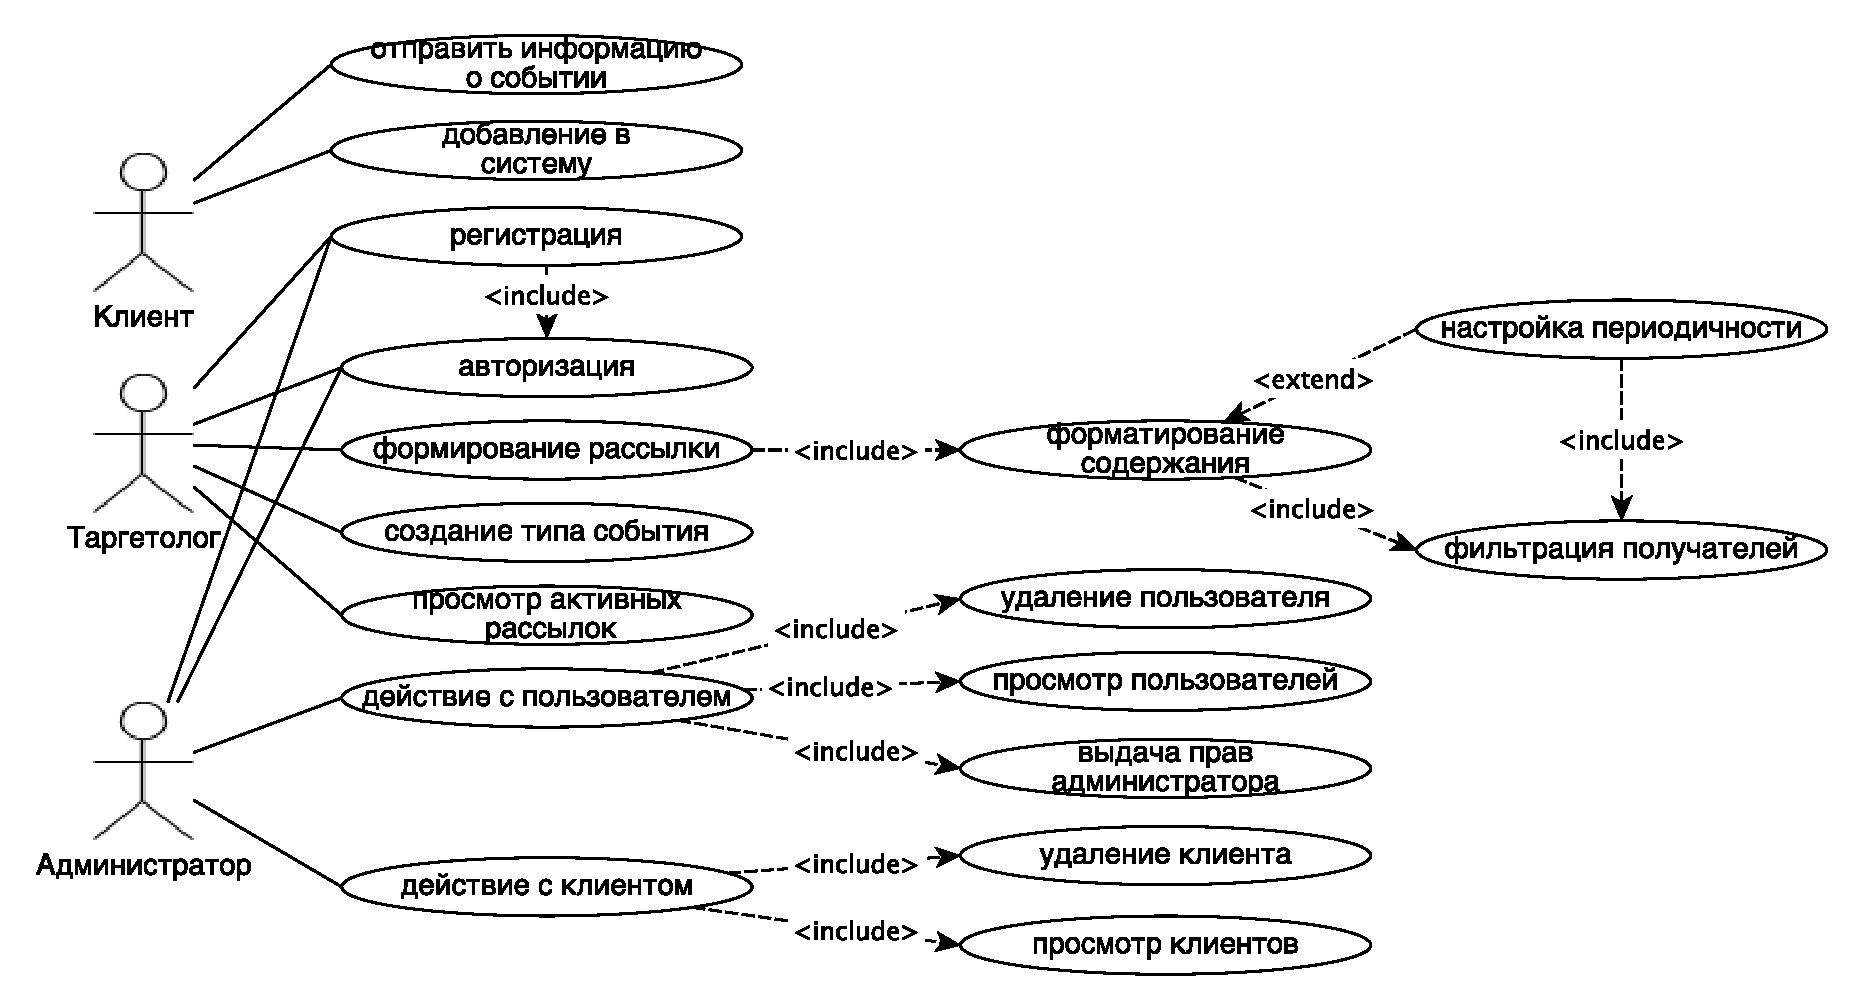
\includegraphics[width=1\linewidth]{./images/use.pdf}
%    \captionof{figure}{Пользовательские сценарии}
%    \label{img:use}
%  \end{tabular}
%\end{table}
%
%\section{Вывод}
%
%В этом разделе был проведён анализ предментой области и обзор существующих решений, обоснована актуальность решаемой продуктом задачи. Также, была формализована задача, пользовательские сценарии и данные. 
%
%Была выбрана реляционная модель данных, как наилучшим образом подходящая для построения системы, подразумевающей нетривиальные связи между сущностями. Отсутствие необходимости изменять структуру данных и возможность исключить дублирование также повлияли на данный выбор.
%
%Для хранения аналитических данных была выбрана колоночная база данных, так как для данного вида информации большую долю запросов будут составлять агрегационные, наиболее оптимально выполнимые в колоночных БД. Для хранения иных данных в работе будет использована строковая БД.
%
%В качестве СУБД была выбрана клиент-серверная, так как данный вариант не накладывает ограничений на объём хранимых данных, и позволяет не манипулировать ненужными в рамках запроса данными.

















 
